\documentclass{article}

\title{Before the rise of um}
\author{Derek Denis and Timothy Gadanidis}

% SIL font
\usepackage{fontspec}
\setmainfont{Charis SIL}

% margins
\usepackage[margin=1in]{geometry}

% bibliography
\RequirePackage[
    backend=biber,
    style=apa,
    sortcites=true,
sorting=nyt]
{biblatex}
\RequirePackage[american]{babel}
\bibliography{beforeum.bib}
\RequirePackage{csquotes}
\RequirePackage[american]{babel}
\DeclareLanguageMapping{american}{american-apa}

% colon postnotes
\renewcommand{\postnotedelim}{%
  \iffieldnums{postnote}
    {\addcolon~}
    {}}
\DeclareFieldFormat{postnote}{#1}
\DeclareFieldFormat{multipostnote}{#1}

% table
\usepackage{booktabs}

% figures
\usepackage{graphicx}

\begin{document}

\maketitle

\section{Introduction}

% TODO: introduction should reflect chapter as a whole

One of the most dramatic discourse-pragmatic changes in twentieth-century
English has progressed under the radar of laypeople and (until recently)
linguists: the rise of \emph{um} as the predominant variant of the `filled
pause' variable (UHM) at the expense of \emph{uh} \parencite{tottie2011,
fruehwald2016, wielingetal2016}.
\textcite[43]{fruehwald2016} documents this ``textbook'' change over 100+ years
of apparent time:
\emph{um} increases incrementally between generations and the rise is led by
women.
In this chapter, we investigate (UHM) at an early stage of change to determine
what triggered the rise of \emph{um}.

\section{Um and uh}

% TODO: brief literature review on what uh/um are, status as words, etc.

[əː] [əːm]

\section{Change in progress}

The rise of \emph{um} has now been described extensively in the variationist and
corpus-linguistic literature, across a number of corpora and speech communities.

% TODO: acton2011

In the British National Corpus, \textcite{tottie2011} observed that \emph{um}
was used more frequently than \emph{uh} by women, younger speakers, and more
educated speakers; men, older speakers and educated speakers used (UHM) more
often overall.
\textcite{fruehwald2016}

% TODO: wielingetal2016

While these accounts demonstrate definitively that a change is underway, an
explanation for the change remains elusive.
What was the trigger for this ``textbook'' change?

% TODO: explain functional expansion hypothesis

In this chapter, we investigate data from before the rise of \emph{um} with the
goal of evaluating the functional expansion hypothesis.

\section{Data}

The data for this study are from the \emph{Farm Work and Farm Life Since 1890}
oral history collection \parencite{denis2016}.
The corpus consists of oral history interviews with 155 elderly farmers,
recorded in 1984.
The corpus covers five regions of Ontario, Canada: Temiskaming, Essex, Dufferin,
Niagara Region, and Eastern Ontario; for this study, speakers from the latter
two regions were considered.
Speaker birth years range from 1891 to 1919, just before \emph{um} began to take
off per \textcite{fruehwald2016}.

We extracted each instance of \emph{uh} and \emph{um} from the transcripts,
excluding unrelated instances such as \emph{uh-oh}.
Tokens from the two much-younger interviewers was also extracted, and analyzed
separately.
The transcription protocol emphasized faithful reproduction of \emph{uh} and
\emph{um}.

\section{Coding}

We coded for the following social factors:
year of birth, gender, and region (Niagara or Eastern Ontario).

To operationalize the functional expansion hypothesis, we coded for utterance
position (initial or non-initial).

% TODO: cliticization

\section{Results}

\subsection{Proportional frequency}

Table~\ref{t:comparison} shows how our data compare with previous communities
analyzed.
The first block summarizes our data from Niagara and Eastern Ontario, as well as
F-INT and M-INT, the two younger interviewers.
The second block summarizes results from previous work on the Switchboard corpus
\parencite{switchboard}, the Fisher corpus \parencite{fisher}, the Philadelphia
Neighborhood Corpus (PNC) \parencite{labovrosenfelder2011}, and the British
National Corpus (BNC) (\citeyear{bnc}).
The numbers for all of these other corpora are drawn from
\textcite{wielingetal2016}.

\begin{table}[ht!]
    \centering
    \begin{tabular}{lrrrrrr}
        \toprule
                    & Raw N       & Raw N       & \%          & Mean              & Mean             & Mean     \\
        Community   & \textit{uh} & \textit{um} & \textit{um} & \textit{uh} /1000 & \textit{um}/1000 & UHM/1000 \\
        \midrule
        Niagara     & 1864        & 357         & 16.1        & 21.3              & 4.1              & 25.4     \\
        E. Ont.     & 1563        & 168         & 9.7         & 22.6              & 2.4              & 25.0     \\
        F-INT       & 321         & 318         & 49.8        & 12.4              & 12.3             & 24.7     \\
        M-INT       & 255         & 51          & 16.7        & 13.2              & 2.6              & 15.8     \\
        \midrule
        Switchboard & ---         & ---         & 28.3        & 22.1              & 7.5              & 29.6     \\
        Fisher      & ---         & ---         & 64.1        & 6.8               & 9.9              & 16.7     \\
        PNC         & ---         & ---         & 27.6        & 13.2              & 4.5              & 17.7     \\
        BNC         & ---         & ---         & 46.1        & 4.5               & 4.3              & 8.8      \\
        \bottomrule
    \end{tabular}
    \caption{Cross-community comparison}
    \label{t:comparison}
\end{table}

As can be seen in the table, \emph{um} is less frequent in our data compared to
the more recent corpora; the female interviewer uses it around half the time,
while the male interviewer's rate is comparable to the farmers'.
Relative frequency of (UHM) taken as a whole is on par with other corpora, but
we are cautious about making such a comparison because each corpus was collected
and transcribed differently \parencite[for related discussion,
see][]{pichler2010}.

Looking at individual speakers' rates, we can see that all speakers use both
\emph{uh} and \emph{um}, but there is no clear pattern by age
(Figure~\ref{fig:indivage}) or gender (Figure~\ref{fig:indivgender}).

% TODO: these figures probably need to be remade in black and white
%       plus there are a lot of visual improvements that could be made

\begin{figure}[htpb]
    \centering
    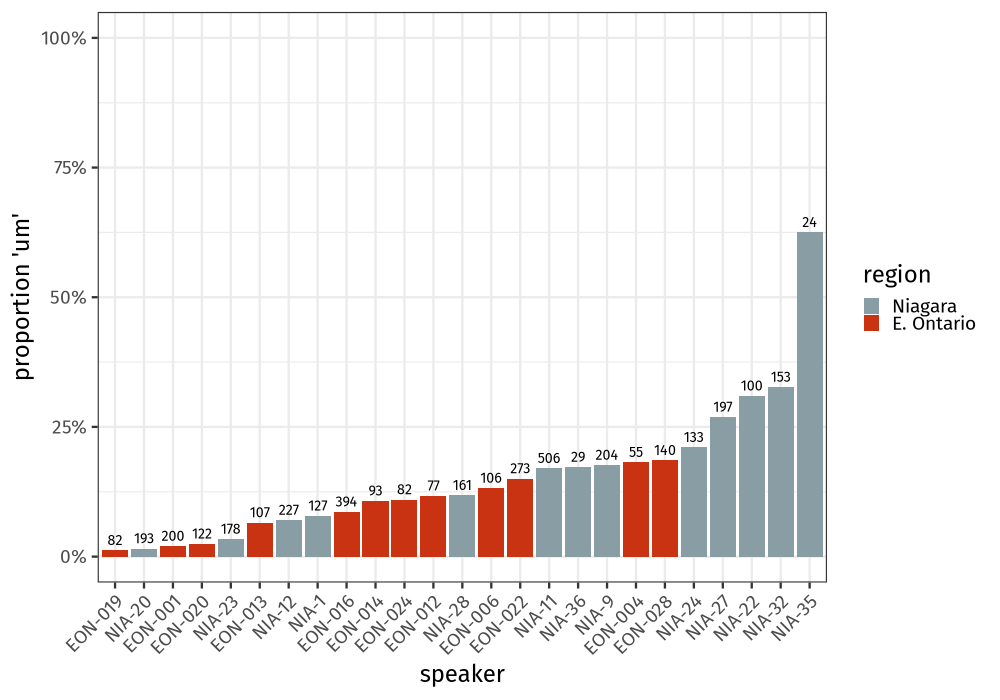
\includegraphics[width=0.8\linewidth]{figures/indivage.png}
    \caption{Proportion \emph{um} per speaker by age.}
    \label{fig:indivage}
\end{figure}

\begin{figure}[htpb]
    \centering
    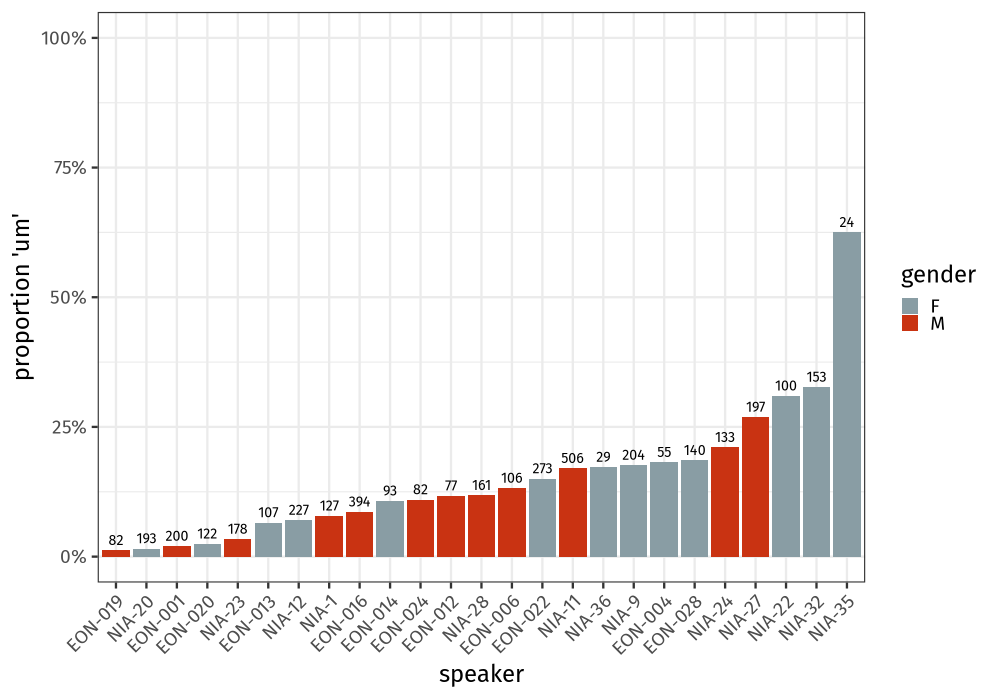
\includegraphics[width=0.8\linewidth]{figures/indivgender.png}
    \caption{Proportion \emph{um} per speaker by gender.}
    \label{fig:indivgender}
\end{figure}

Figure~\ref{fig:apparenttime} shows the proportion of \emph{um} in apparent
time.
There is a modest trend upward over time.

\begin{figure}[htpb]
    \centering
    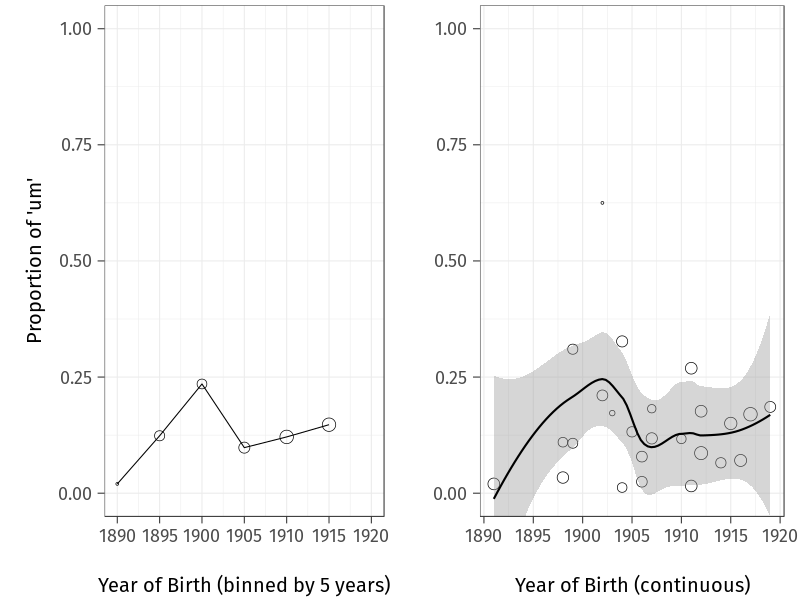
\includegraphics[width=0.8\linewidth]{figures/apparenttime.png}
    \caption{Proportion \emph{um} in apparent time.}
    \label{fig:apparenttime}
\end{figure}

Figure~\ref{fig:apparentgender} shows the pattern when splitting speakers by
gender.
Starting around 1905, women use \emph{um} slightly more than men do.

\begin{figure}[htpb]
    \centering
    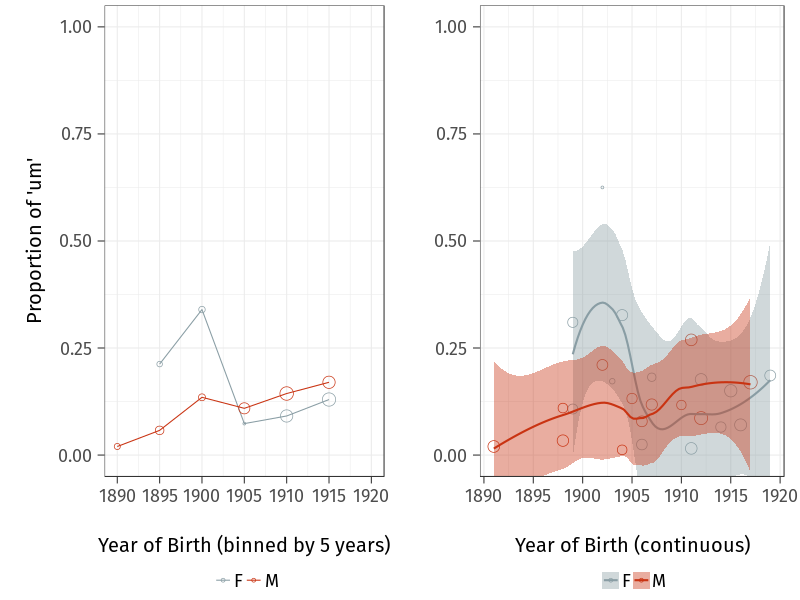
\includegraphics[width=0.8\linewidth]{figures/apparentgender.png}
    \caption{Proportion \emph{um} in apparent time, by gender.}
    \label{fig:apparentgender}
\end{figure}

Figure~\ref{fig:apparentposition} shows the pattern when splitting tokens by
position (initial vs.\ non-initial).
Starting around 1905, \emph{um} is used more frequently in initial position than
in non-initial position.

\begin{figure}[htpb]
    \centering
    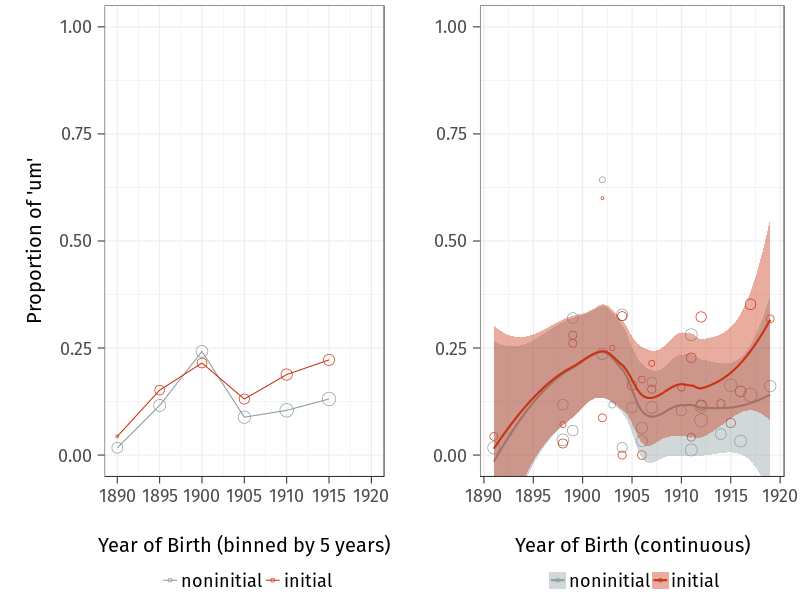
\includegraphics[width=0.8\linewidth]{figures/apparentposition.png}
    \caption{Proportion \emph{um} in apparent time, by position.}
    \label{fig:apparentposition}
\end{figure}

Figure~\ref{fig:apparentclitic} shows the pattern when splitting tokens by
cliticization with \emph{and} or \emph{but} and position.

\begin{figure}[htpb]
    \centering
    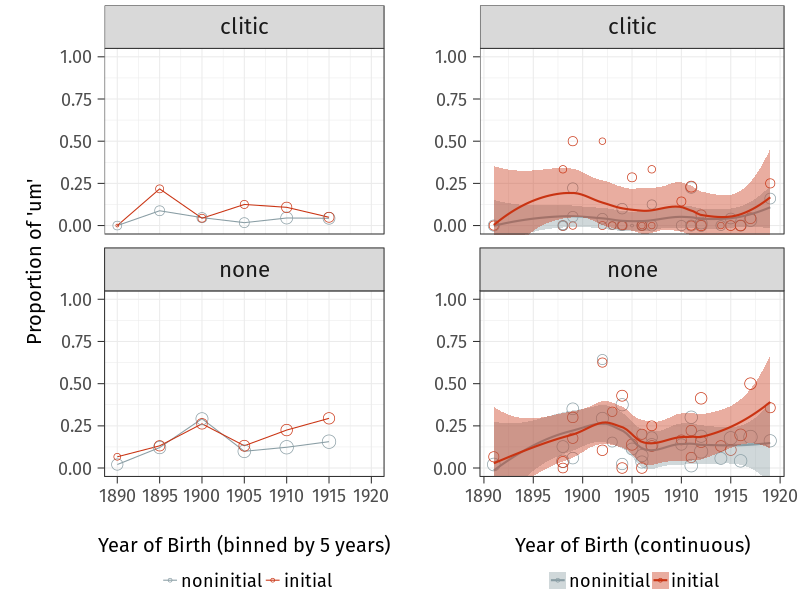
\includegraphics[width=0.8\linewidth]{figures/apparentclitic.png}
    \caption{Proportion \emph{um} in apparent time, by position and
    cliticization.}
    \label{fig:apparentclitic}
\end{figure}

Figure~\ref{fig:farmertree} shows a conditional inference tree for all farmers.

\begin{figure}[htpb]
    \centering
    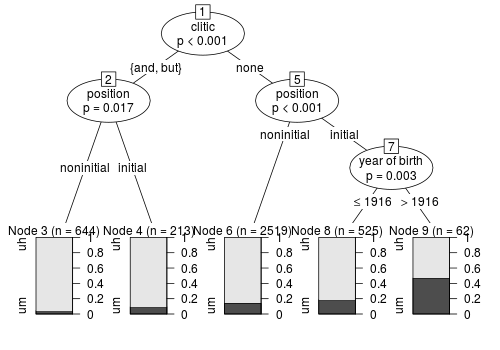
\includegraphics[width=0.8\linewidth]{figures/ctree.png}
    \caption{Conditional inference tree for farmers.}
    \label{fig:farmertree}
\end{figure}

Figure~\ref{fig:interviewertree} shows a conditional inference tree for the two
interviewers.

\begin{figure}[htpb]
    \centering
    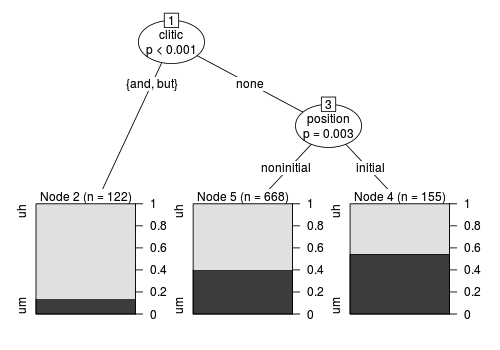
\includegraphics[width=0.8\linewidth]{figures/ctreeint.png}
    \caption{Conditional inference tree for interviewers.}
    \label{fig:interviewertree}
\end{figure}

Taken together, these results show the beginning of the change toward \emph{um}
that has been observed by other researchers.
While other work has shown that women lead this change, in our data, older women
actually use more \emph{um} than the younger women.

Looking at internal factors, we can see that cliticized forms, like
\emph{and-uh}, favour \emph{uh}.
There is some evidence for positional divergence, possibly consistent with a new
utterance-initial discourse function that favours \emph{um}
\parencite[cf.][, who found no turn-positional difference]{fruehwald2016}.
Conditional inference trees confirm that the internal constraints persist with
the younger speakers, while their baseline \emph{um} rate is higher.

\subsection{Relative frequency}

\textcite{fruehwald2016} tests the hypothesis that functional expansion
triggered the rise of um by considering changes to the relative frequency of
variants over time (e.g., frequency of \emph{um} or \emph{uh} per 10~000 words).
When a new discourse-pragmatic function emerges, we expect that these functions
would add to the relative frequency of the feature, and if the new function is
restricted to one variant, the relative frequency of that variant should rise,
with little change to the relative frequency of the other variant.
In other words, we expect a fishtail pattern as with \emph{computer} and
\emph{typewriter} over time: once \emph{computer} gained its contemporary
meaning, its relative frequency grew additively as that meaning became more
frequent.
This is illustrated in Figure~\ref{fig:fishtail} \parencite[Figure 3
from][]{fruehwald2016}: looking at the proportion of \emph{computer} over
\emph{typewriter} (left graph), \emph{computer} appears to replace
\emph{typewriter} over time; but looking at the relative frequency of each word
(right graph), it's clear that \emph{typewriter} remained stable as
\emph{computer} took off.

\begin{figure}[htpb]
    \centering
    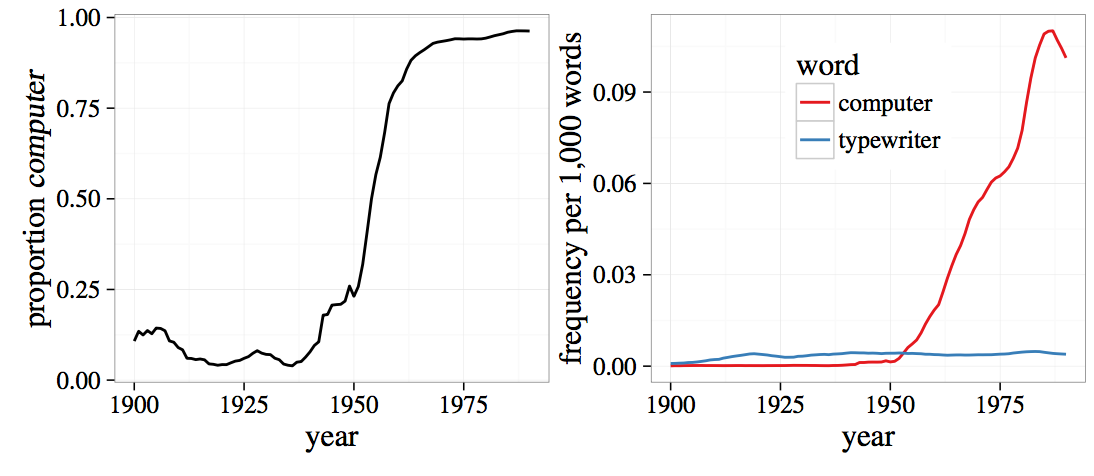
\includegraphics[width=0.8\linewidth]{figures/fishtail.png}
    \caption{Proportional frequency and relative frequency of \emph{computer}
    and \emph{typewriter} \parencite[Figure 3 from][]{fruehwald2016}.}
    \label{fig:fishtail}
\end{figure}

\printbibliography

\end{document}
